\begin{flushleft} % sætter tekststarten i venstre marginside.
\doublespacing


Vi ønsker at se hvordan metoden startRules og konstruktøren for StartField klassen fungerer. startRules metoden skal sørge for, at give spilleren en startbonus på 2M når de passerer start og konstruktøren kaldes når der laves et StartField objekt, der skal bruges i spillebrættets array som det første felt.
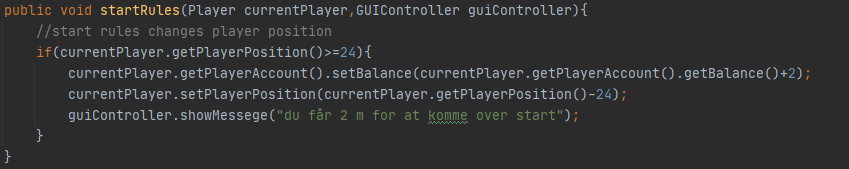
\includegraphics[width=1\textwidth]{Report/figures/startRules.PNG}~\\[0cm] 
Figur 6.1. Metoden startRules() i Rules klassen.
\addlinespace
Først kigger på vi på startRules metoden. Vi kan se at, metoden tager en spiller og en GUIController som parameter. \\
Spilleren i parametret er spilleren der har turen. Her tjekker den med et if-statement, om spillerens position er større end brættets størrelse(24). 
Hvis den er det, tilføjes der 2M på spillerens konto som det første.
Dernæst vil spillerens position blive ændret, så den passer ind i brættets størrelse. Dermed fungerer selve spillebrættet som en cirkel, der starter forfra når man passerer det sidste felt i spillebrættets array i koden. Til sidst sørger GUIControlleren for, at der kommer en besked, om at spilleren har passeret start og modtager en bonus, som kan ses i selve GUI'en når man kører spillet.

\newpage
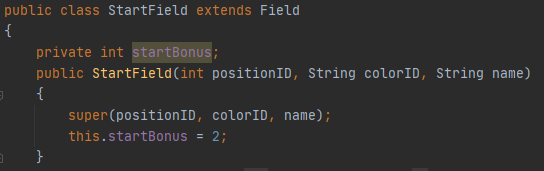
\includegraphics[width=1\textwidth]{Report/figures/StartField constructor.PNG}~\\[0cm] 
Figur 6.2. Konstruktøren i StartField klassen.
\addlinespace
Konstruktøren tager et positionID som heltal, en colorID som tekststreng og et navn også som tekststreng, som parametre.
Inde i selve konstruktøren kan vi se, at den kalder disse via super-metoden. 
Dette er muligt med nedarvning. Hvis man ser på øverste linje hvor klassen bliver lavet, kan man se, at der står "extends Field".
Dette betyder, at den arver fra klassen Field, heriblandt konstruktøren i Field klassen, hvor disse parametre også er krævet.
Med nedarvning, kan man blandt andet undgå at gentage en masse kode, og hvis der skal ændres, kan dette gøres ét enkelt sted.
\newpage
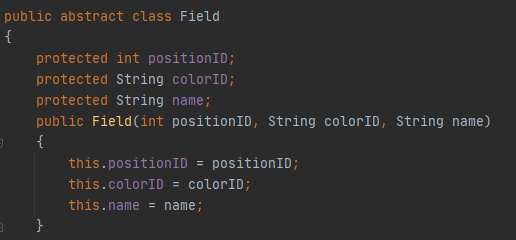
\includegraphics[width=1\textwidth]{Report/figures/Field constructor.PNG}~\\[0cm] 
Figur 6.3. Konstruktøren i Field klassen
\addlinespace
I figur 6.3 kan man se Field klassen som bliver nedarvet i StartField klassen. Her kan man blandt andet se konstruktøren der bliver nedarvet, hvor parametrene går igen, og er årsagen til at man ikke skal kalde dem individuelt i StartFields konstruktør.
Man kan også se, at der står "abstract" foran "class Field". Dette betyder, at man ikke kan kalde på klassen Field eller lave objekter af denne klasse.
Den eksisterer udelukkende, så andre klasser kan nedarve fra den, og centralisere koden der skal påvirke alle de nedarvede klasser.
\end{flushleft}